% Grounded AutoML-Agent -- paper skeleton.
% Uses only standard packages so it compiles anywhere (Overleaf, TeX Live, MiKTeX).
% To submit to a venue, replace the \documentclass/preamble with the venue style file
% (e.g. icml2026.sty or neurips_2026.sty); the section files do not need to change.

\documentclass[11pt]{article}

\usepackage[margin=1in]{geometry}
\usepackage[T1]{fontenc}
\usepackage[utf8]{inputenc}
\usepackage{lmodern}
\usepackage{microtype}
\usepackage{amsmath,amssymb}
\usepackage{booktabs}
\usepackage{graphicx}
\usepackage{xcolor}
\usepackage{algorithm}
\usepackage{algpseudocode}
\usepackage[numbers]{natbib}
\usepackage[hidelinks]{hyperref}
\usepackage{cleveref}
\usepackage{tikz}
\usetikzlibrary{arrows.meta,positioning}

\graphicspath{{figures/}}
\newcommand{\todo}[1]{\textcolor{red}{[TODO: #1]}}
% Include a figure produced by evaluation/analysis.py, or a placeholder if it does not exist yet.
\newcommand{\resultfigure}[2]{%
  \IfFileExists{figures/#1.pdf}{\includegraphics[width=#2]{#1}}%
  {\fbox{\parbox[c][4cm][c]{#2}{\centering\small Figure \texttt{#1} is generated by\\ \texttt{python -m evaluation.analysis}}}}}

\title{Grounded AutoML-Agent: Budget-Aware Multi-Fidelity Verification\\and Experience Memory for Scalable LLM-Driven AutoML}
\author{%
  Abhinandh A \quad Jason Bobby \quad Pranav Hariharan \quad Sajish Sajan Varghese \quad Aniketh S\\[2pt]
  {\small 2024BCD0009 \quad 2024BCD0013 \quad 2024BCD0005 \quad 2024BCS0001 \quad 2024BCS0049}\\[4pt]
  Indian Institute of Information Technology Kottayam}
\date{}

\begin{document}
\maketitle

\begin{abstract}
Multi-agent LLM frameworks such as AutoML-Agent automate the full machine-learning pipeline from a natural-language request. Their efficiency relies on \emph{pseudo-execution}: before any code runs, an agent predicts how well each candidate plan will perform, and the most promising plan is implemented. We show that these predictions are \todo{poorly / moderately} calibrated (Spearman $\rho = $ \todo{x}) and that plan selection built on them is fragile, especially with inexpensive backbone models. We propose \textbf{Grounded AutoML-Agent}, which (i)~replaces pseudo-execution-based verification with budget-aware successive halving over nested data subsamples, and (ii)~adds an experience memory that recalls plans, observed scores and bug fixes from past runs on similar datasets. Built on a scalable execution substrate (Parquet ingest, fixed stratified splits, gradient-boosted trees with early stopping, out-of-core text models), the system runs on a single CPU machine with a free-tier Gemini model and handles datasets of millions of rows. Across \todo{N} datasets, grounding improves the comprehensive score by \todo{x} at equal wall-clock budget, and memory reduces LLM calls by \todo{y\%} over a task sequence. \todo{One sentence on the backbone result (RQ4).}
\end{abstract}

\section{Introduction}
\label{sec:intro}

Automated machine learning (AutoML) promises models without expert effort, yet classical systems still require users to specify the task, the data pipeline and the search space \citep{feurer2015autosklearn,erickson2020autogluon}. Large language model (LLM) agents lower this barrier further: AutoML-Agent \citep{trirat2025automlagent} turns a natural-language request into a trained model through a team of specialised agents, retrieval-augmented planning and multi-stage verification.

A key design choice of AutoML-Agent is \emph{pseudo-execution}. Data and Model agents reason about each candidate plan and predict its performance, and the Manager implements the plan that looks best, which avoids training every candidate. This saves compute, but the predictions are never checked against reality. The authors also report that quality collapses with smaller backbone models, precisely where predictions should be least reliable.

\paragraph{Contributions.}
\begin{itemize}
  \item We measure, for the first time, the calibration of LLM pseudo-execution in agentic AutoML (RQ1).
  \item We introduce \emph{grounded verification}: budget-aware successive halving over nested data subsamples, which selects plans on observed rather than predicted performance (RQ2).
  \item We add an \emph{experience memory} that recalls measured outcomes and bug fixes from similar past runs (RQ3).
  \item We show that the combined system runs end to end on a real 8.9M-row dataset with a free-tier model on a laptop (RQ4), and we harden it into a usable system: a pre-training data audit, human-in-the-loop control, skew-free model serving and time-series forecasting. Code, web UI and evaluation harness accompany the paper.
\end{itemize}

\section{Related Work}
\label{sec:related}

\paragraph{AutoML systems.} Auto-sklearn \citep{feurer2015autosklearn} and AutoGluon \citep{erickson2020autogluon} search over pipelines and ensembles with fixed search spaces. Multi-fidelity methods such as successive halving and Hyperband \citep{jamieson2016successive,li2018hyperband} allocate compute to promising configurations using cheap low-fidelity evaluations.

\paragraph{LLM agents for data science.} DS-Agent \citep{guo2024dsagent} uses case-based reasoning over Kaggle solutions; SELA \citep{chi2024sela} combines LLM agents with Monte Carlo tree search over executed experiments. AutoML-Agent \citep{trirat2025automlagent} covers the full pipeline with retrieval-augmented planning and pseudo-execution.

\paragraph{Our position.} We keep AutoML-Agent's agentic planning, replace its unverified pseudo-execution with multi-fidelity \emph{grounding} borrowed from classical AutoML, and add a memory of \emph{measured} outcomes. \todo{Expand with memory/experience-replay agents and LLM calibration literature.}

\section{Method}
\label{sec:method}

\subsection{Pipeline overview}
The pipeline follows AutoML-Agent (\Cref{fig:pipeline}). A Prompt Agent parses the request into a task specification, which is verified against a statistical profile of the data. The data is converted to Parquet, split once into fixed train/validation/test partitions and audited. The Manager retrieves knowledge and proposes $P$ candidate plans; Data and Model agents analyse each plan and predict its score $\hat{s}_p$. Where AutoML-Agent selects the plan with the best \emph{predicted} score, we select on \emph{observed} scores (grounded verification). An optional human gate can approve, pick or edit the selected plan. An Operation Agent implements it from a working template, and implementation verification checks the requirements on the held-out test split, triggering revisions if needed. Finished runs produce a model card, a memory record and a servable model.

\begin{figure}[t]
  \centering
  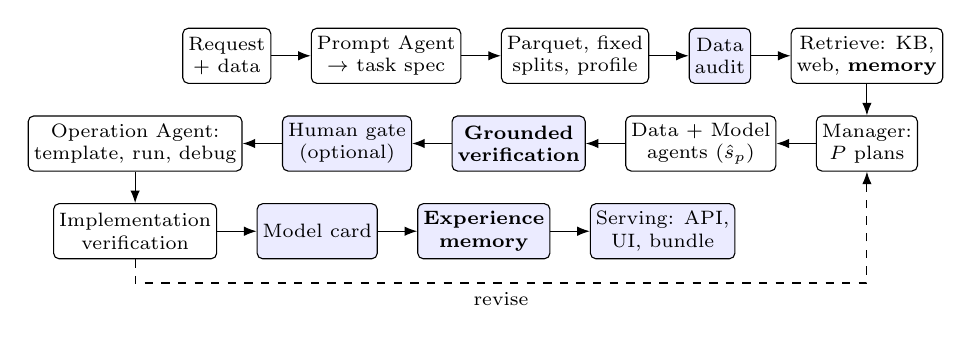
\begin{tikzpicture}[
      node distance=4mm and 5mm,
      box/.style={draw, rounded corners=2pt, align=center, font=\scriptsize, minimum height=7mm, inner sep=2pt},
      new/.style={box, fill=blue!8},
      arr/.style={-{Latex[length=1.6mm]}}]
    \node[box] (req) {Request\\+ data};
    \node[box, right=of req] (parse) {Prompt Agent\\$\to$ task spec};
    \node[box, right=of parse] (prep) {Parquet, fixed\\splits, profile};
    \node[new, right=of prep] (audit) {Data\\audit};
    \node[box, right=of audit] (ret) {Retrieve: KB,\\web, \textbf{memory}};
    \node[box, below=of ret] (plan) {Manager:\\$P$ plans};
    \node[box, left=of plan] (agents) {Data + Model\\agents ($\hat{s}_p$)};
    \node[new, left=of agents] (ground) {\textbf{Grounded}\\\textbf{verification}};
    \node[new, left=of ground] (human) {Human gate\\(optional)};
    \node[box, left=of human] (op) {Operation Agent:\\template, run, debug};
    \node[box, below=of op] (verify) {Implementation\\verification};
    \node[new, right=of verify] (card) {Model card};
    \node[new, right=of card] (mem) {\textbf{Experience}\\\textbf{memory}};
    \node[new, right=of mem] (serve) {Serving: API,\\UI, bundle};
    \draw[arr] (req) -- (parse); \draw[arr] (parse) -- (prep); \draw[arr] (prep) -- (audit);
    \draw[arr] (audit) -- (ret); \draw[arr] (ret) -- (plan); \draw[arr] (plan) -- (agents);
    \draw[arr] (agents) -- (ground); \draw[arr] (ground) -- (human); \draw[arr] (human) -- (op);
    \draw[arr] (op) -- (verify); \draw[arr] (verify) -- (card); \draw[arr] (card) -- (mem);
    \draw[arr] (mem) -- (serve);
    \draw[arr, dashed] (verify.south) -- ++(0,-3mm) -| node[pos=0.25, below, font=\scriptsize] {revise} (plan.south);
  \end{tikzpicture}
  \caption{Pipeline. White: stages inherited from AutoML-Agent. Shaded: our additions. Bold: the two research contributions.}
  \label{fig:pipeline}
\end{figure}

\subsection{Grounded verification}
Let $\mathcal{D}_\text{train}$ have $n$ rows, each with an independent draw $u_i \sim \mathcal{U}[0,1)$. The subsample at fidelity $r$ is $S_r = \{i : u_i < r/n\}$, so $S_r \subseteq S_{r'}$ for $r \le r'$. Rung $k$ trains every surviving plan on $S_{r_k}$ with $r_k = \min(r_0 g^k, n)$ and scores it on a fixed validation slice, keeping the best $\lceil P_k/\eta \rceil$ plans (\Cref{alg:grounding}). The test split is never used for selection: when implementation verification triggers a revision, attempts are also compared on validation scores, and only the chosen attempt's test score is reported.

\begin{algorithm}[t]
\caption{Budget-aware grounded verification}
\label{alg:grounding}
\begin{algorithmic}[1]
\Require plans $\mathcal{P}$, rows $n$, $r_0$, growth $g$, keep ratio $\eta$, remaining time $T$
\State $\mathcal{S} \gets \mathcal{P}$;\; $k \gets 0$
\While{$|\mathcal{S}| > 1$ \textbf{or} $k = 0$}
  \State $r_k \gets \min(r_0 g^k, n)$
  \If{$k > 0$ \textbf{and} $\bar t_{k-1}\, (r_k/r_{k-1})\, |\mathcal{S}| > T$} \textbf{break} \EndIf
  \For{$p \in \mathcal{S}$} \State $s_p \gets \textsc{TrainAndScore}(p, S_{r_k})$ \EndFor
  \State $\mathcal{S} \gets$ top-$\lceil |\mathcal{S}|/\eta \rceil$ of $\mathcal{S}$ by $s_p$;\; $k \gets k+1$
  \If{$r_k = n$} \textbf{break} \EndIf
\EndWhile
\State \Return plans ranked by (last rung reached, observed score)
\end{algorithmic}
\end{algorithm}

\subsection{Experience memory}
Each run stores dataset meta-features $m \in \mathbb{R}^d$ (size, column-type mix, missingness, class count and imbalance), all candidate plans with predicted and observed scores, the selected plan's test score, error$\to$fix pairs, and whether a human overrode the agents' choice. For a new task, the $k$ nearest runs of the same task type under a weighted Euclidean distance are rendered as planning knowledge, in the spirit of meta-learning warm starts \citep{feurer2015autosklearn}; matching error signatures surface past fixes to the Operation Agent.

\subsection{Scalable execution substrate}
Datasets are converted once to Parquet; profiling uses a lazy engine with approximate distinct counts; a fixed stratified train/validation/test split per target is shared by all plans, fidelities and baselines. Training templates use gradient-boosted trees with native categoricals and early stopping \citep{ke2017lightgbm}, and out-of-core hashing models for large text corpora. Scripts run in a supervised subprocess with time and memory limits.

\subsection{Platform extensions}
Four extensions turn the research prototype into a usable system; they are not part of the comparison with the paper but are evaluated by the test suite.

\paragraph{Data audit and model card.} Selecting on measured scores makes target leakage \citep{kaufman2012leakage} more dangerous: a leaking column always wins. Before planning, a deterministic audit drops identifier-like discrete columns, columns whose names echo the target, mostly-empty and constant columns, and any single feature that predicts the target with AUC, accuracy or $R^2 \ge 0.98$ on a shuffled holdout; it also counts exact train/test duplicates by row hashing. After training, a model card \citep{mitchell2019modelcards} reports feature importances, per-class metrics, calibration or residuals, computed through the serving code path.

\paragraph{Human in the loop.} Runs can pause after grounded verification so a user can approve, pick or edit a plan (and optionally the script), with a timeout fallback, cancellation that kills the training process tree, and resumption after a server restart onto the plans the user reviewed.

\paragraph{Model serving.} Training templates record their feature preparation (dtypes, category levels, column roles) in the model bundle, and one standalone module replays it for the REST API, the CLI, the model card and an exported bundle, avoiding training/serving skew \citep{sculley2015debt}; a test checks that served predictions reproduce the training script's test score.

\paragraph{Time-series forecasting.} A forecasting task type uses date-aligned temporal splits whose grounding rungs are suffix windows (the most recent data), a global direct multi-horizon LightGBM model on lag, rolling and calendar features computed strictly from the past, and seasonal-naive and ETS baselines; every model is scored with a rolling-origin backtest \citep{hyndman2021fpp3}, and served forecasts start from each series' recent history.

\section{Experimental Setup}
\label{sec:setup}

\paragraph{Datasets.} The tabular and text datasets of \citet{trirat2025automlagent} (Banana Quality, Software Defects, Crab Age, Ecommerce Text), each with a constraint-free and a constraint-aware instruction, and large-scale datasets: a synthetic 5M-row conversion task, HIGGS (11M), NYC Taxi fares and Amazon Polarity. \todo{Table of dataset statistics.}

\paragraph{Metrics.} Success rate (SR, graded 0/0.5/1), normalized performance score (NPS; RMSLE for regression) and comprehensive score $\text{CS} = 0.5\,\text{SR} + 0.5\,\text{NPS}$, as in the original paper; calibration by Spearman $\rho$, top-1 hit rate and MAE between predicted and observed scores; cost as wall time, LLM calls and tokens.

\paragraph{Variants and baselines.} \texttt{paper} (pseudo verification, no memory), \texttt{grounded}, \texttt{memory}, \texttt{full} (both), and \texttt{full\_fused} (single analysis call per plan). Baselines: Gemini zero-shot single script, and Optuna + LightGBM with the same wall-clock budget.

\paragraph{Protocol.} Fixed seeded 70/15/15 splits; three seeds; leave-one-dataset-out memory; equal budgets per comparison. Backbone: \todo{Gemini model ids per role}. Hardware: \todo{CPU, RAM}.

\section{Results}
\label{sec:results}

\paragraph{RQ1: Calibration of pseudo-execution.} \todo{Report $\rho$, top-1 hit rate and MAE (Table~\ref{tab:calibration}); discuss Figure~\ref{fig:calibration}.}

\begin{figure}[t]
  \centering
  \resultfigure{fig_calibration}{0.45\linewidth}
  \caption{Predicted vs.\ observed validation scores at the first grounding rung.}
  \label{fig:calibration}
\end{figure}

\begin{table}[t]
  \centering
  \caption{Calibration of pseudo-execution predictions. \todo{fill from \texttt{table\_calibration.md}.}}
  \label{tab:calibration}
  \begin{tabular}{lrrrr}
    \toprule
    Variant & Groups & Spearman $\rho$ & Top-1 hit & MAE \\
    \midrule
    \todo{grounded} & & & & \\
    \bottomrule
  \end{tabular}
\end{table}

\paragraph{RQ2 and RQ4: Grounding and backbone.} \todo{Main table: SR/NPS/CS/time/calls per variant and baseline (Table~\ref{tab:main}); Figure~\ref{fig:cs}.}

\begin{table}[t]
  \centering
  \caption{Main results (mean over datasets, prompts and seeds). \todo{fill from \texttt{table\_main.md}.}}
  \label{tab:main}
  \begin{tabular}{lrrrrr}
    \toprule
    Variant & SR & NPS & CS & Wall (s) & LLM calls \\
    \midrule
    paper & & & & & \\
    grounded & & & & & \\
    full & & & & & \\
    zero-shot & & & & & \\
    Optuna+LightGBM & & & & & \\
    \bottomrule
  \end{tabular}
\end{table}

\begin{figure}[t]
  \centering
  \resultfigure{fig_cs_by_variant}{0.6\linewidth}
  \caption{Comprehensive score by variant; dots are individual tasks.}
  \label{fig:cs}
\end{figure}

\paragraph{RQ3: Experience memory.} \todo{LLM calls and CS over the task sequence (Figure~\ref{fig:memory}).}

\begin{figure}[t]
  \centering
  \resultfigure{fig_memory_curve}{0.55\linewidth}
  \caption{LLM calls per run over the task sequence, without (dashed) and with (solid) memory.}
  \label{fig:memory}
\end{figure}

\section{Ablations and Analysis}
\label{sec:ablations}

\todo{Grounding schedule sensitivity ($r_0$, $g$, $\eta$); effect of \texttt{AGENT\_FUSION} on quality and cost; single vs.\ role-split backbone; template-fallback rate; scaling of wall time with dataset size; cost of grounding relative to full training of every plan.}

\section{Limitations}
\label{sec:limitations}

\paragraph{Scope of the evaluation.} Our experiments use two large tabular datasets, one real (Microsoft Malware Prediction) and one synthetic, with a single seed per configuration, on one laptop and a free-tier backbone. This is enough to characterise behaviour at scale, but not to make statistically strong claims across task families; the paper's own benchmark datasets (Kaggle) and three seeds remain to be run with the provided configuration (\texttt{paper\_tabular.json}).

\paragraph{Method.} Grounding adds training cost, which is bounded by the schedule and the budget but not negligible on very large data. The memory benefits only related tasks and could propagate past mistakes, although records carry observed failures. The data audit uses fixed thresholds; a feature that is legitimately almost deterministic of the target would be dropped.

\paragraph{Modalities.} We cover tabular classification and regression, text classification and time-series forecasting; image and graph tasks are left to future work.

\paragraph{Backbone drift.} Hosted LLMs evolve and free-tier quotas fluctuate (our runs met overload and quota errors and fell back across model versions), so exact numbers may drift. We mitigate this by logging the model used for every call and caching all responses. Public benchmark datasets may appear in pre-training data.

\section{Conclusion}
\label{sec:conclusion}

\todo{Summarise findings for RQ1--RQ4 and the practical takeaway: measure, don't predict, when compute allows it; and let the system remember what it measured.}


\bibliographystyle{plainnat}
\bibliography{refs}

\appendix
\section{Implementation Details}
\label{app:implementation}

\paragraph{Agents and prompts.} Six system prompts live in \texttt{backend/src/automl\_agent/prompts}: Prompt Agent (request $\to$ task specification), Manager (retrieval-augmented planning of $P$ plans in one structured call), Data Agent and Model Agent (per-plan analysis with a predicted score), Plan Analyst (both analyses in one call when \texttt{AGENT\_FUSION} is on) and Operation Agent (edits a rendered working template; repairs failures given the error and past fixes). Every response is constrained by a JSON schema derived from the corresponding Pydantic model.

\paragraph{Backbone and rate limits.} The \emph{smart} role (Manager planning and Operation Agent code) uses \texttt{gemini-3.8-flash} with fallbacks \texttt{gemini-3.7-flash}, \texttt{gemini-3.6-flash}, \texttt{gemini-3.5-flash} on overload (HTTP 503) or quota errors; the \emph{fast} role (Prompt Agent parsing and the per-plan Data/Model/Plan-Analyst analysis) uses \texttt{gemini-3.1-flash-lite}. Requests are limited to 5 (smart) and 15 (fast) per minute with at most 2 in flight, retried with exponential backoff that honours the server's \texttt{retryDelay}, and cached on disk keyed by model, prompt and seed. Web knowledge comes from Gemini's Google Search grounding when quota allows.

\paragraph{Model registry.} Plans must choose a family from a per-task registry, filtered by training-set size:
\begin{center}
\small
\begin{tabular}{ll}
\toprule
Task & Families (row limit) \\
\midrule
Tabular (both) & LightGBM, XGBoost, HistGradientBoosting, SGD (any size); random forest, extra trees ($\le$1M); \\
 & gradient boosting ($\le$200k); $k$-NN ($\le$100k); RBF SVM ($\le$20k) \\
Classification & + logistic regression ($\le$2M) \\
Regression & + ridge (any size), lasso ($\le$2M) \\
Text & TF-IDF + logistic regression / linear SVM / complement NB / SGD ($\le$1M); hashing + SGD (any size) \\
Forecasting & direct global LightGBM; seasonal-naive; ETS \\
\bottomrule
\end{tabular}
\end{center}

\paragraph{Grounding defaults.} $r_0 = 20{,}000$ rows, growth $g = 4$, keep ratio $\eta = 2$, validation cap $100{,}000$ rows; with $P = 3$ plans and millions of training rows this gives rungs of 20k (3 plans) and 80k rows (2 plans) before the full-data run of the winner.

\paragraph{Splits and audit.} 70/15/15 train/validation/test, stratified for classification and contiguous date blocks for forecasting, seeded and cached per target. The audit drops discrete columns that are $\ge 90\%$ unique with an identifier-like name or $\ge 99\%$ unique otherwise, columns whose names echo the target, constant columns and columns $\ge 80\%$ missing, and single features reaching AUC, accuracy or $R^2 \ge 0.98$ on a shuffled 80/20 holdout of up to 10k rows.

\paragraph{Execution.} Scripts run in a subprocess with a 30-minute timeout and a memory watchdog at 80\% of physical RAM; on repeated failure (3 debug attempts) the unmodified template runs as a safety net. Every run records its full configuration, including model ids and all settings, in the run's \texttt{config}.

\section{Reproducibility}
\label{app:reproducibility}

All experiments are produced by \texttt{python -m evaluation.run\_benchmark} with the configs in \texttt{backend/evaluation/configs} (\texttt{local\_large.json} for the results in this paper); tables and figures by \texttt{python -m evaluation.analysis}; forecasting numbers by \texttt{python -m evaluation.forecasting\_benchmark}. LLM responses are cached per seed, so re-running a config reproduces the same LLM outputs. The Microsoft Malware Prediction training set is the Kaggle competition file \texttt{train.csv} (8{,}921{,}483 rows), converted once to Parquet with \texttt{automl\_agent.tools.ingest}.


\end{document}
